\section{Resultados}

\begin{frame}{O simulador}

  \begin{center}
  {\huge \textbf{Demonstração do simulador.}}
  \end{center}

  \begin{center}
  
\includegraphics[height=\dimexpr5\textheight/14\relax]{figuras/engines}
  \end{center}

\end{frame}

\begin{frame}[allowframebreaks]{Arquitetura}

  \begin{figure}[t]
    \centering
    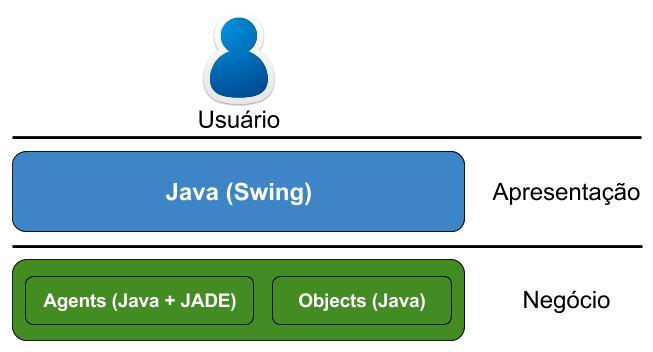
\includegraphics[height=\dimexpr8\textheight/14\relax]{figuras/arquitetura_geral}
    \caption{Modelo arquitetural do sistema}
  \end{figure}

%\end{frame}

%\begin{frame}{Arquitetura}

  \begin{figure}[t]
    \centering
    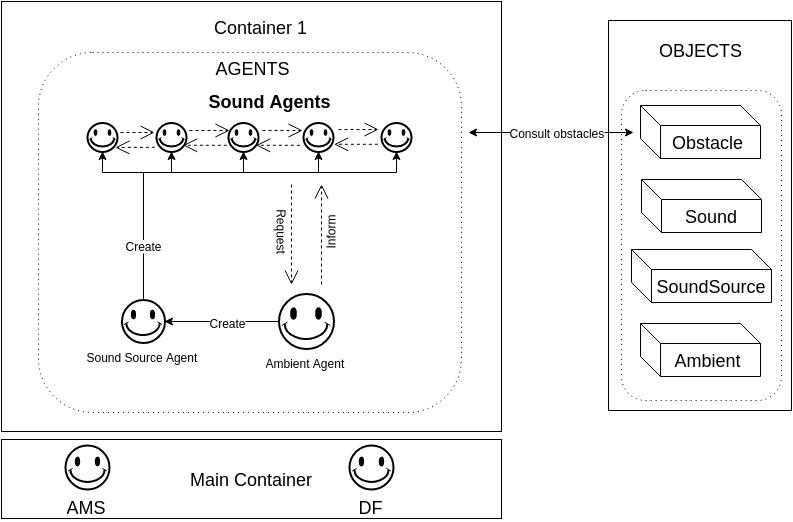
\includegraphics[height=\dimexpr9\textheight/14\relax]{figuras/arquitetura}
    \caption{Máquina de raciocínio do simulador acústico}
  \end{figure}

\end{frame}

\begin{frame}{Testes unitários e cobertura de código}

  \begin{figure}[t]
    \centering
    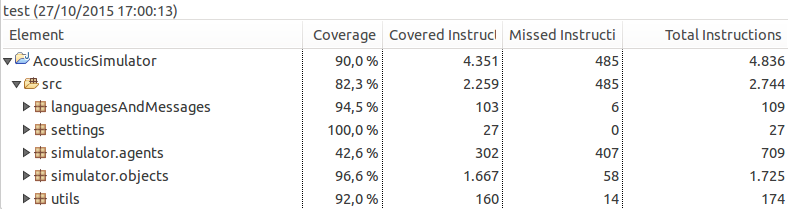
\includegraphics[height=\dimexpr6\textheight/14\relax]{figuras/cobertura}
    \caption{Cobertura de código}
  \end{figure}

\end{frame}

\begin{frame}[allowframebreaks]{Métricas de qualidade de código fonte}

Dentre as métricas suportadas pelo Analizo, \citeonline{meirelles} seleciona um subconjunto representativo, pois foi constatado que muitas delas eram redundantes por medir prioridades muito correlacionadas.
\linebreak
\linebreak
\begin{enumerate}
\item Conexões aferentes, ou ACC, uma medida de \textbf{acoplamento}.
\linebreak
\item Média da \textbf{complexidade ciclomática} dos métodos, ou ACCM.
\linebreak
\item Média do \textbf{tamanho dos métodos}, ou AMLOC.
\linebreak
\item Média do \textbf{número de parâmetros por métod}o, ou ANPM.

\newpage

\item \textbf{Profundidade na árvore de herança}, ou DIT.
\linebreak
\item \textbf{Número de métodos}, ou NOM.
\linebreak
\item \textbf{Número de atributos públicos}, ou NPA.
\linebreak
\item \textbf{Complexidade estrutural}, ou SC, uma medida que combina acoplamento (CBO) e coesão (LCOM4).
\end{enumerate}

\newpage

As métricas colhidas foram analisadas qualitativamente, baseando-se nos intervalos sugeridos no trabalho de \citeonline{kalibro}.
\linebreak
  \begin{figure}[t]
    \centering
    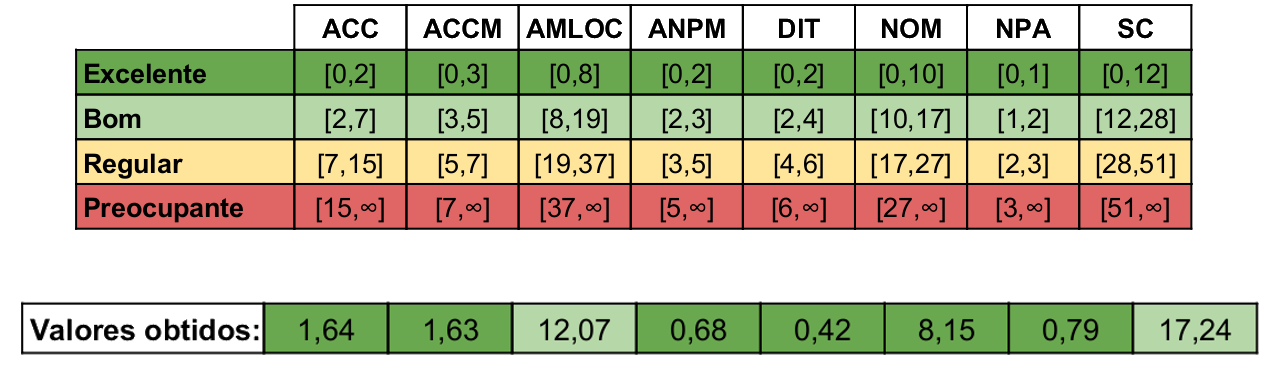
\includegraphics[height=\dimexpr7\textheight/14\relax]{figuras/Analise_estatica}
    \caption{Análise estática do código fonte}
  \end{figure}
\end{frame}

\begin{frame}[allowframebreaks]{Comparação entre os cenários de uso avaliados}

Configurações e especificações técnicas do ambiente:
\begin{itemize}
\item Processador Intel Core i7, modelo 2630QM de 2Ghz 
\item 6 Gb de memória ram 
\item Ubuntu 14.04.3 LTS, 64 bits 
\item Java 1.8.0\_66
\end{itemize}

\begin{table}[]
\centering
\caption{Cenários avaliados}
\label{cenarios}
\begin{tabular}{|l|c|c|c|}
\hline
\textbf{Dados do ambiente} & \multicolumn{1}{l|}{\textbf{Cenário 1}} & \multicolumn{1}{l|}{\textbf{Cenário 2}} & \multicolumn{1}{l|}{\textbf{Cenário 3}} \\ \hline
Largura              & 4 m                  & 3 m                & 25 m            \\
Comprimento          & 4 m                  & 7 m                & 20 m            \\
Altura               & 3 m                  & 4 m                & 6  m            \\
Absorção média       & 9 \%                 & 10 \%              & 20 \%           \\ \hline
\end{tabular}
\end{table}
  
  \begin{figure}[t]
    \centering
    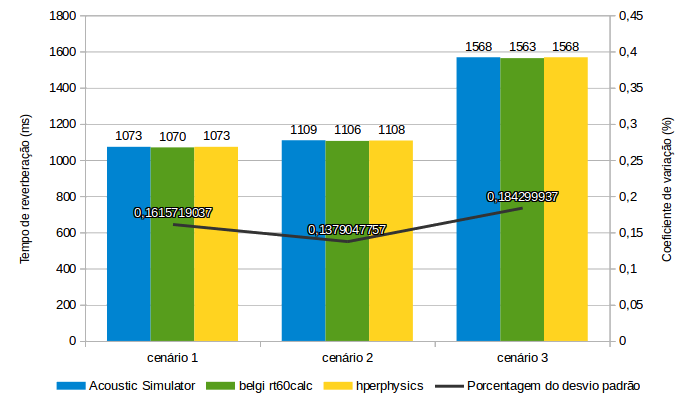
\includegraphics[height=\dimexpr10\textheight/14\relax]{figuras/comparacao}
    \caption{Tempo de reverberação dos simuladores por cenário.}
  \end{figure} 
\end{frame}